\documentclass[12pt,twoside,english]{article}
\usepackage[utf8]{inputenc}

%%%%%%%%%%%%%%%%%%%%%%%%%%%%%%%%%%%%%%%%%%%%%%%%%%%%%%%%%%%%%%%%%%%%%%%
%% template for II2202 proposal
%% original 2020.08.28
%% revised  
%%%%%%%%%%%%%%%%%%%%%%%%%%%%%%%%%%%%%%%%%%%%%%%%%%%%%%%%%%%%%%%%%%%%%%%
%

%%% Local Variables:
%%% mode: latex
%%% TeX-master: "."
%%% End:

%%TC:ignore
\usepackage[paper=a4paper,dvips,top=1.5cm,left=1.5cm,right=1.5cm,
    foot=1cm,bottom=1.5cm]{geometry}


\usepackage{todonotes}          %to provide inline and margin notes
%\usepackage[T1]{fontenc}
%%\usepackage{pslatex}
\renewcommand{\rmdefault}{ptm} 
\usepackage{mathptmx}
\usepackage[scaled=.90]{helvet}
\usepackage{courier}
%
\usepackage{bookmark}

\usepackage{fancyhdr}
\pagestyle{fancy}

%%----------------------------------------------------------------------------
%%   pcap2tex stuff
%%----------------------------------------------------------------------------
 %%\usepackage[dvipsnames*,svgnames]{xcolor} %% For extended colors
 %%\usepackage{tikz}  %% Already loaded
 %%\usetikzlibrary{arrows,decorations.pathmorphing,backgrounds,fit,positioning,calc,shapes}

%% \usepackage{pgfmath}	% --math engine
%%----------------------------------------------------------------------------
%% \usepackage[latin1]{inputenc}
\usepackage[utf8]{inputenc} % inputenc allows the user to input accented characters directly from the keyboard
\usepackage[english]{babel}
%% \usepackage{rotating}		 %% For text rotating
\usepackage{array}			 %% For table wrapping
\usepackage{graphicx}	                 %% Support for images
\usepackage{float}			 %% Suppor for more flexible floating box positioning
\usepackage{color}                       %% Support for colour 
\usepackage{mdwlist}
%% \usepackage{setspace}                 %% For fine-grained control over line spacing
%% \usepackage{listings}		 %% For source code listing
%% \usepackage{bytefield}                %% For packet drawings
\usepackage{tabularx}		         %% For simple table stretching
%%\usepackage{multirow}	                 %% Support for multirow colums in tables
\usepackage{dcolumn}	                 %% Support for decimal point alignment in tables
\usepackage{url}	                 %% Support for breaking URLs
\usepackage[perpage,para,symbol]{footmisc} %% use symbols to ``number'' footnotes and reset which symbol is used first on each page
\usepackage[binary-units=true]{siunitx} %% to be able to use binary units
\newcommand{\SIadj}[2]{\SI[number-unit-product={\text{-}}]{#1}{#2}}

%% \usepackage{pygmentize}           %% required to use minted -- see python-pygments - Pygments is a Syntax Highlighting Package written in Python
%% \usepackage{minted}		     %% For source code highlighting

%% \usepackage{hyperref}		
\usepackage[all]{hypcap}	 %% Prevents an issue related to hyperref and caption linking
%% setup hyperref to use the darkblue color on links
%% \hypersetup{colorlinks,breaklinks,
%%             linkcolor=darkblue,urlcolor=darkblue,
%%             anchorcolor=darkblue,citecolor=darkblue}

%% Some definitions of used colors
\definecolor{darkblue}{rgb}{0.0,0.0,0.3} %% define a color called darkblue
\definecolor{darkred}{rgb}{0.4,0.0,0.0}
\definecolor{red}{rgb}{0.7,0.0,0.0}
\definecolor{lightgrey}{rgb}{0.8,0.8,0.8} 
\definecolor{grey}{rgb}{0.6,0.6,0.6}
\definecolor{darkgrey}{rgb}{0.4,0.4,0.4}
%% Reduce hyphenation as much as possible
\hyphenpenalty=15000 
\tolerance=1000

%% useful redefinitions to use with tables
\newcommand{\rr}{\raggedright} %% raggedright command redefinition
\newcommand{\rl}{\raggedleft} %% raggedleft command redefinition
\newcommand{\tn}{\tabularnewline} %% tabularnewline command redefinition

%% definition of new command for bytefield package
\newcommand{\colorbitbox}[3]{%
	\rlap{\bitbox{#2}{\color{#1}\rule{\width}{\height}}}%
	\bitbox{#2}{#3}}

%% command to ease switching to red color text
\newcommand{\red}{\color{red}}
%%redefinition of paragraph command to insert a breakline after it
\makeatletter
\renewcommand\paragraph{\@startsection{paragraph}{4}{\z@}%
  {-3.25ex\@plus -1ex \@minus -.2ex}%
  {1.5ex \@plus .2ex}%
  {\normalfont\normalsize\bfseries}}
\makeatother

%%redefinition of subparagraph command to insert a breakline after it
\makeatletter
\renewcommand\subparagraph{\@startsection{subparagraph}{5}{\z@}%
  {-3.25ex\@plus -1ex \@minus -.2ex}%
  {1.5ex \@plus .2ex}%
  {\normalfont\normalsize\bfseries}}
\makeatother

\setcounter{tocdepth}{3}	%% 3 depth levels in TOC
\setcounter{secnumdepth}{5}
%% Acronyms
\usepackage[acronym, nopostdot]{glossaries}
\glsdisablehyper
\makeglossaries

\renewcommand{\headrulewidth}{0pt}
%%%%%%%%%%%%%%%%%%%%%%%%%%%%%%%%%%%%%%%%%%%%%%%%%%%%%%%%%%%%%%%%%%%%
%% End of preamble
%%%%%%%%%%%%%%%%%%%%%%%%%%%%%%%%%%%%%%%%%%%%%%%%%%%%%%%%%%%%%%%%%%%%

\newacronym{AR}{AR}{augmented reality}

% Keywords command
\providecommand{\keywords}[1]
{
  \small	
  \textbf{\textit{Keywords:}} #1
}

\title{Trade-offs Between Immersion and Energy Consumption With Automatic Naturalistic Lighting in Augmented Reality}
\author{
        \textsc{Stefano Formicola}
            \qquad
        \textsc{Christoph Albert Johns}
        \mbox{}\\
        \normalsize
            \texttt{formico}
        \textbar{}
            \texttt{cajohns}
        \normalsize
            \texttt{@kth.se}
}
\date{\today}


\lhead{II2202, Fall 2020, Period 1-2}
%% or \lhead{II2202, Fall 2020, Period 1}
\chead{Draft Project Report}
\rhead{\date{\today}}

\makeatletter
\let\ps@plain\ps@fancy 
\makeatother

\setlength{\headheight}{15pt}
\begin{document}

\maketitle


\begin{abstract}
\label{sec:abstract}

This research project proposes and tests a method to investigate the effect of automatic naturalistic lighting in \gls{AR} applications on immersion and on energy consumption.
A simple open-source card-matching game is modified to implement and control the corresponding rendering setting as provided by Apple's \gls{AR} \gls{API} RealityKit and tested with a small sample of users.
A within-subject research design with a small convenience sample is chosen to measure immersion through the \gls{IEQ} while overall \gls{CPU} usage is monitored and logged for both test conditions in randomized order.
A Mann-Whitney-U-test is used to test for significant differences in immersion and \gls{CPU} usage between both conditions.
The pre-test shows that the proposed method is generally appropriate to test the hypothesized relationships.
For a large-scale study, usability issues of the sample application should be resolved for more reliable measures or another application could be considered.
Additionally, it should be considered whether the \gls{IEQ} should be replaced with a questionnaire that is more specific to \gls{AR} applications.
The preliminary results seem to suggest that neither immersion nor \gls{CPU} usage are significantly affected by automatic naturalistic lighting, although a larger scale study is required for a more meaningful account.

\end{abstract}

%TC:ignore
\keywords{Augmented reality, Lighting, Immersion, Energy consumption}
%TC:endignore
\clearpage

\selectlanguage{english}
\tableofcontents

\section*{List of Acronyms and Abbreviations}
\label{list-of-acronyms-and-abbreviations}
\renewcommand{\glossarysection}[2][]{} %% skip the title
\printglossary[type=\acronymtype, nonumberlist]

\clearpage
\section{Introduction}
\label{sect:introduction}

% What is the problem?
In recent years, increasingly advanced features for \gls{AR} have become readily available to developers and designers in the form of easy-to-use \glsplural{API}.
Apple's \gls{AR} \gls{API} RealityKit, for example, has enabled creators to easily add occlusion, video textures, and shared states to their \gls{AR} applications \cite{apple_realitykit_2020-1}.
One of the especially notable features implemented by this \gls{API} has been real-time light estimation \cite{apple_arlightestimate_2020}.
Applications that enable this feature gain access to information about a scene's lighting with every video frame that is delivered to the current session \cite{apple_arlightestimate_2020}.
This information can then be used to apply dynamic shading to virtual objects matching the real-world lighting conditions \cite{apple_arlightestimate_2020}.
Apple's RealityKit \gls{API} enables this feature by default and-–depending on the available hardware–-uses one or multiple probes in the scene to measure and estimate this so called "environment lighting".
The resulting lighting estimate is then applied to the virtual objects in the scene \cite{apple_disablearenvironmentlighting_2020}.
To achieve this naturalistic lighting, camera-sensor data is continuously processed and evaluated to estimate and approximate the environment's lighting conditions and dynamically add the appropriate shading to the objects in a scene~\cite{apple_arlightestimate_2020,apple_disablearenvironmentlighting_2020}.
Depending on the scene and lighting conditions, this can be a computationally intensive process~\cite{steed_constructing_2016}.
Enabling this feature could, therefore, lead to increased scene realism at the cost of decreased energy efficiency.
This research aims at illuminating the relationship between immersion and energy impact in deploying automatic naturalistic lighting, thus empowering developers and designers to decide the most appropriate feature sets for their applications considering both user experience and sustainability aspects.
While there have been user-based studies evaluating visual characteristics of \gls{AR} objects, this particular aspect of automatic naturalistic lighting appears not to have been examined yet.


% What are the major contributions?
Examining the problem statement, two eventual outcomes of our project are possible:
If we find a trade-off between immersion and energy consumption, designers and developers should be recommended to avoid continuous \gls{AR} light estimation in order to free resources for either alternative uses or to extend battery life.
If we find no trade-off, developers and designers can be responsibly encouraged to implement the feature in order to enhance overall immersion.
Each outcome could be considered a worthwhile contribution to the field of \gls{AR} and immersion research.
The expected deliverables for our project are: an example \gls{AR} application to measure immersion levels and monitor energy consumption; a pre-tested and evaluated method (setup, procedure, and analysis) for a full-scale study; an indication for the results of a full-scale study.


% What are the research questions?
Overall, we will explore the following questions:

\begin{description}
    \item[RQ1.] Do users perceive a difference in immersion between enabled and disabled automatic naturalistic lighting?
    \item[RQ1a.] If they perceive a difference, are the participants able to tell that lighting is the cause?
    \item[RQ2.] How does enabling automatic naturalistic lighting affect \gls{CPU} usage?
\end{description}

Energy consumption will be measured in terms of \gls{CPU} usage for two major reasons.
First, because there is no dedicated \gls{GPU} in the mobile devices we will be testing, so the \gls{CPU} will handle all processing related to the \gls{AR} experience.
And second, because CPU usage can very finely be measured on the test device in contrast to general energy consumption.
While we are aware that we will only be able to test the proposed method on a small scale, we hypothesize the following outcomes for a full-scale experiment.


% What are the hypotheses?
As will be further explained in section \ref{sect:related_works}, scene realism is positively correlated with presence and thereby immersion.
That is why we expect the lighting condition that more closely matches the scene's natural environment to lead to higher levels of immersion, resulting in the following hypothesis:

\begin{description}
    \item[H1.] Users experience higher immersion levels when automatic naturalistic lighting is enabled.
\end{description}

Because the difference between both conditions lies in a salient visual feature which affects \gls{AR} objects' color and reflections, we expect not only the indirect measure of immersion as assessed through the \gls{IEQ} to be affected.
We instead hypothesize that users will recognize the difference between both conditions and will be able to articulate how they differ without support from the examiner.
This leads us to this hypothesis:

\begin{description}
    \item[H1a.] Users are able to tell that the lighting was different between both runs of the experiment.
\end{description}

Finally, regarding the energy impact of naturalistic lighting, we expect the computationally intensive continuous probing and estimation of the \gls{AR} scenes environment lighting to lead to higher levels of overall \gls{CPU} usage:

\begin{description}
    \item[H2.] \gls{CPU} usage is higher when automatic naturalistic lighting is enabled.
\end{description}


\section{Related Works}
\label{sect:related_works}

Our research project builds on two main lines of research: prior works evaluating the relationship between visual characteristics of \gls{AR} objects and user experience (e.g.~\cite{gabbard_effects_2006}) and research on the approximation of natural lighting conditions within virtual scenes in augmented reality (e.g.~\cite{aittala_inverse_2010}).
While there has been extensive research on the effect of design decisions on several aspects of user experience in digital games~\cite{johnson_validation_2018} -- even in \gls{AR} games in a few instances (e.g.~\cite{georgiou_development_2017}) -- the effect of lighting and more specifically automatic naturalistic lighting in \gls{AR} games on immersion seems not to have been examined yet.

While several aspects of the experience when playing videos games in general and \gls{AR} games in particular have been defined and measured as well (see~\cite{dey_systematic_2018, dunser_survey_2008} for overviews), we chose to investigate the effect of automatic naturalistic lighting on immersion because--in contrast to, for example, \textit{flow}~\cite{csikszentmihalyi_flow_1990}--it is independent from optimal experience, which our method will not be able to produce, and very likely to relate to visual presentation and, therefore, lighting~\cite{jennett_measuring_2008}.
As Witmer and Singer argue, "scene realism" is one of the governing factors for presence in virtual environments~\cite{witmer_measuring_1998}, which in turn affects how immersive a virtual environment appears~\cite{jennett_measuring_2008}.
We reason that automatic naturalistic lighting enhances this sense of realism and will therefore affect users' sense of immersion.


\section{Method}
\label{sect:method}

We modified an existing open source mobile \gls{AR} game for our experiment to test immersion levels and energy consumption during the usage.
Players' immersion has been measured through the \gls{IEQ}, while Xcode's Developer Tools has been used to measure \gls{CPU} usage over time.
Because of its popularity across countries and languages, we considered the game \textit{Memory} or \textit{Concentration}, in which players have to remember the order and color of different cards, a valid candidate for the experiment.

The implementation has been done for iOS devices and developed on Apple's \gls{IDE} Xcode using the ARKit and RealityKit frameworks \gls{API}.
The user interface included a toggle button invisible to the player but useful to enable and disable the automatic naturalistic lighting feature for the two runs of the experiment.

The experiment consisted of one three-minute session of gameplay for each condition, with and without the automatic naturalistic lighting, per subject.
During each phase of the experiment a non-invasive data collection was performed using Xcode Developer Tools' \emph{Instruments} to measure the computational load.

Finally, we measured subjects' immersion levels for each condition using the \gls{IEQ} proposed by Jennett et al.~\cite{jennett_measuring_2008}.

The project used a within-subjects design to empirically test two different lighting conditions in an experiment setting and analyze the results using statistical methods.
In the following, the targeted participant profile, data collection, analysis and study procedure are described.

\subsection{Participants}
\label{sect:participants}

The participants were recruited via an opportunity sample and were -- due to the difficulties and restrictions regarding gatherings of people during the COVID-19 pandemic -- mostly international students living at KTH Main Campus.
To limit the effect of novelty on immersion levels, participants were required to have had played a card-matching game similar to the sample game before.
It was, however, not required that they have played a digital version of this game before taking part in the experiment.
To further mitigate the effect of novelty, participants were required to have experienced an \gls{AR} scene on a mobile handheld device before.
Overall, seven participants took part in this study.
They had an average age of 24.7 (SD = 1.60), ranging from 23 to 28 years.
All seven participants were male.

\subsection{Data collection}
\label{sect:data_collection}

During each run of the experiment, the \gls{IDE} Xcode and more specifically its \textit{Instruments} feature~\cite{apple_xcode_2020} have been used to log the test device's \gls{CPU} usage in three second intervals, according to Apple's type definitions~\cite{apple_system_2020}.
While there exist a more general power metric that can be logged through the same application~\cite{apple_energy_2020-1}, that metric is discrete and inelastic towards enabled and disabled automatic naturalistic lighting and was, therefore, not used.
We discussed and decided not to have participants think aloud during their app usage to avoid unwanted effects on their experience and, thus, immersion~\cite{van_den_haak_retrospective_2003}.
After each run, participants were asked to fill out the \gls{IEQ} (see Appendix \ref{sect:ieq}) to measure their levels of immersion dependent on the lighting treatment.
After the second run, participants have been additionally asked about their general experience using the application and to elaborate on any differences they noticed between both runs.
While alternatives such as tracking eye movement or measuring reaction times could also have been used to measure immersion~\cite{jennett_measuring_2008}, we chose a questionnaire approach as the most economical option that still has satisfactory precedence in literature~\cite{boyle_engagement_2012}.
If a participant mentioned one of the words "light", "lighting", "color", or "contrast" while answering these questions, the difference in lighting was considered as noticed by the user.

\subsection{Data analysis}
\label{sect:data_analysis}

After the above data have been successfully gathered, we conducted a statistical analysis regarding the participants' immersion levels and the \gls{CPU} usage between both lighting conditions using Student's two-sample \textit{t}-test in Python to check for significant differences.
We chose this measure as it can be considered quite robust even with small and extremely small ($ N \leq 5 $) sample sizes~\cite{de_winter_using_2013} and because it was used by Jennett et al. in their original experiments~\cite{jennett_measuring_2008}.
However, the \textit{t}-test's assumption of normal distribution was not met, therefore we proceeded conducting a Mann-Whitney U-test to compare the two conditions following the example of Nordin et al.~\cite{nordin_attention_2013} in their immersion experiments.
Additionally, we reported the results of the interview.

We were aware that both the results of our analysis of variance and the of our interviews could not be used to infer knowledge about either the effect of automatic naturalistic lighting on immersion or energy consumption.
Rather, the analysis was carried out in order to evaluate the chosen methods and to illustrate how such analysis should have been done if the same study was carried out on a larger scale.

\subsection{Procedure}
\label{sect:procedure}

We modified an open-source \gls{AR} card-matching game~\cite{cobb_maxxfrazerrealitykit-cardflip_2020} to include an option to enable and disable automatic naturalistic lighting using RealityKit's \textit{.disableAREnvironmentLighting} render option for a repeated measures study design.

Before the start of the experiment participants have been informed about the collection of data regarding the device activity and their questionnaire answers after both runs of the game, moreover their right to withdraw from the experiment at any time was clarified as well as the possibility to ask the deletion of data. The purpose of the experiment has been stated to the participants only in general terms as "investigating immersion in \gls{AR} games" to avoid influencing their perception of the scene by directing their attention towards lighting. 
They were asked to fill in a Google Forms document their name and surname followed by the date of the experiment and check the boxes corresponding to their willing to share the data and confirming they have been informed of the above stated experiment details.

The game has been presented to participants on an Apple iPad in an indoor setting with controlled lighting where participants were asked to complete as many rounds of the card-matching game for each of the two lighting conditions as they could, before they were interrupted after three minutes and the render option changed for the second run.
The order of render options has been randomized (through a number generator) to improve reliability and participants were not informed about the currently active render option to avoid biases.

The sample application was chosen due to its simplicity in functionality and visual presentation as well as general familiarity, thereby reducing the risk of errors in use or unwanted effects on immersion due to scene complexity or novelty.
To further negate this risk and to address the concerns brought up by Jennett et al.~\cite{jennett_measuring_2008} regarding the effect of prior experience on immersion, participants were given a trial period with a third lighting condition: disabled automatic naturalistic lighting and an added point light above the scene.
The goal stated to the participants was to complete the game as fast as possible and with as few errors as possible, following the study design of Jennett et al.~\cite{jennett_measuring_2008}.
This should have allowed for a more challenging experience across player ability levels and, therefore, increased flow~\cite{csikszentmihalyi_flow_1990} and thereby general immersion levels as well as reduced overall variance in immersion~\cite{jennett_measuring_2008}.
The first run were considered started after the participants indicated that they were ready for the experiment to begin.
After the experiment, participants were debriefed and fully informed about the purpose of the study and given the opportunity to withdraw their consent.
The duration of the experiment per participant was 20 minutes.

\section{Results}
\label{sect:results}

Our results can be divided into three parts: (1) the indicative results of our statistical analysis, (2) our own observations when developing and using the tools we devised, (3) our observations of the study participants, and (4) the feedback and comments of our study participants.
Since the main contribution of this study lies in the tooling that we developed and pre-tested for a full-scale study, let us first let us at the secondary contribution: the indicative results of our statistical analysis.

All statistical analysis was performed using Python 3.8.3 with the packages Pandas 1.1.4 and SciPy 1.5.4.
All visualizations were created using Seaborn 0.11.0.
The immersion scores per question according to the \gls{IEQ} were calculated as ranging from a 1 for strongly disagree to a 5 for strongly agree.
Scores for positively formulated questions were added, while scores for negatively formulated questions were subtracted to calculate the overall immersion score per participant and condition.
Overall \gls{CPU} usage per timestamp was calculated by adding the \gls{CPU} usage percentages for all activity kinds with the same timestamp.
Since the System CPU Percentage Engineering Type~\cite{apple_system_2020} has a range from 0\% to 100\% multiplied by the number of \gls{CPU} cores in the given device, this can result in values exceeding 100\% (or 1 as in the formatting of our analysis).
Contrary to our first hypothesis \textbf{H1}, overall immersion scores did not differ significantly between both conditions (Mann-Whitney $ U = 18.5 $, $ p = 0.241 $) with the mean overall immersion score for the automatic naturalistic lighting disabled condition even slightly exceeding the enabled condition with scores of 74.7 (SD = 7.3) and 76.0 (SD = 6.6) respectively (see Figure \ref{fig:immersion_plot}).

\begin{figure}[h]
    \centering
    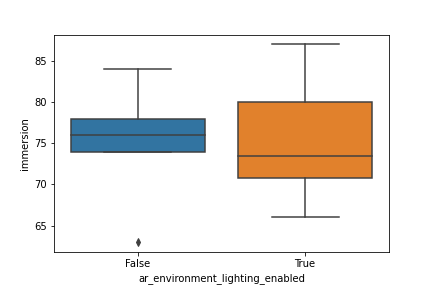
\includegraphics[width=0.5\textwidth]{imgs/immersion_plot}
    \caption{Immersion scores for the disabled and enabled conditions in our small pre-test ($ N = 7 $).}
    \label{fig:immersion_plot}
\end{figure}

Regarding hypothesis \textbf{H1a}, there was no indication whether most participants in a full-scale study would notice a difference between both conditions as three of the seven participants in our pre-test stated they had not noticed any distinction.
Within the group of participants that had answered to have noticed a difference, the immersion scores between automatic naturalistic lighting enabled and disabled did not differ significantly (Mann-Whitney $ U = 4.0 $, $ p = 0.155 $) with mean immersion scores of 76.3 (SD = 4.9) and 76.0 (SD = 11.4) respectively.
Finally, contrary to our hypothesis \textbf{H2}, mean \gls{CPU} usage did not significantly differ between both conditions (Mann-Whitney $ U = 16.0 $, $ p = 0.405 $) with 61.8\% (SD = 6.7\%) mean overall \gls{CPU} usage in the disabled condition and 63.1\% (SD = 6.6\%) in the enabled condition.
However, as can be seen in Figure \ref{fig:cpu_raw_plot}, the distributions of overall \gls{CPU} usage did appear different.
The enabled condition resulted in a significantly higher overall \gls{CPU} usage even in our small pre-test (Mann-Whitney $ U = 53272.5 $, $ p < 0.05 $).

\begin{figure}[h]
    \centering
    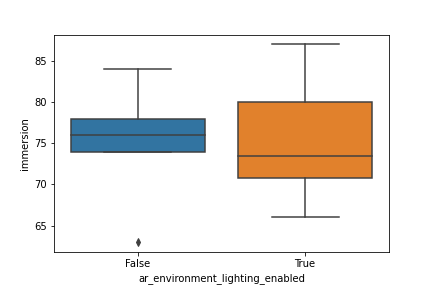
\includegraphics[width=0.5\textwidth]{imgs/cpu_raw_plot}
    \caption{Overall \gls{CPU} usage for the disabled and enabled conditions in our small pre-test ($ N = 7 $). The overall \gls{CPU} usage can exceed 1 for devices with more than one \gls{CPU} core (range from 0 to number of cores) as specified in the corresponding data type definition of the logging software~\cite{apple_system_2020}.}
    \label{fig:cpu_raw_plot}
\end{figure}

While conducting the pre-test, we experienced some difficulties with our chosen software.
The modified sample application as well as the monitoring and logging software chosen had reliability issues that hindered the data gathering process.
In one of the experiments, logging of the \gls{CPU} usage suddenly stopped after circa 1.5~min.
While other data such as network events that were logged automatically by the software could still be accessed, \gls{CPU} data was non-retrievable.
In another experiment, the logging software crashed after requesting to stop and save the recording.
Here again, the \gls{CPU} data wan non-retrievable.
The sample application, similarly, experienced some issues that seemed to relate to the Xcode \gls{IDE}.
In one experiment, the application failed to exit through the software and had to be manually shut down.
Regarding less severe concerns, the sample application appeared to lack in terms of its feedback mechanisms.
During multiple experiments, the probing phase (i.e. the phase during which the application gathers information about the environment, specifically to find a horizontal plane to use as an anchor for the virtual objects of the scene) which was indicated by an overlay with instructions to slowly move the device was exited without placing the virtual objects in an appropriate time frame.
No inherent error or pattern to this behavior could be identified.
This lead to multiple restarts of the application which delayed several runs of the experiment.
The Google Forms questionnaire developed for data gathering did pose any significant challenges when used by the testers.
The Jupyter notebook developed for data analysis, similarly, did not lead to any significant difficulties.

During the experiments, several participants experienced difficulties when interacting with the sample application.
Since the application does support scaling and positioning during the setup phase for increased usability but does not save these settings, the virtual cards were displayed in the original scale and position after each successful game resulting in visible irritation by the participants.
Additionally, the participants seemed to experience some discomfort holding the test device as multiple participants started frequently adjusting their grip during the second run of the experiment.
One participant even rested the device on a table to avoid having to hold it.
It was, furthermore, noticeable that all participants moved the device during the trial phase of the experiment and some at the beginning of the first run, but all stopped moving the device altogether eventually.
They instead remained in a fixed position once a comfortable posture was discovered and only interacted with the application by tapping the screen.
One participant tried multiple different postures, positions, distances, and orientations during the trial phase but, just as the other participants, stopped this exploratory behavior completely once the first run started.
Finally, multiple participants were briefly distracted during one or both runs of the experiment by noises or other people in the test environment.
One participant attempted to start a conversation with the testers during one of the runs which was denied but still interrupted the run.

Our discussions with the participants revealed that the reliability and usability issues we observed matched the participants' experiences.
Multiple participants noted that they were irritated by the inconsistent scale and position of the virtual objects.
Three participants stated unprompted that the device was uncomfortable to hold for the duration of the experiment due to its size and sharp edges.
The sample application was generally accepted.
Two participants noted that its simplicity might limit the potential immersion and that the lack of more complex objects and reflections might result in generally smaller differences in immersion between both runs.
They, furthermore, suspected that this would make it harder for participants to notice any differences between both runs.
The results would additionally be affected by the study design itself.
Some participants noted that asking about the overall experience and any differences between both runs of the experiment would lead to biased answers since it provoked answers even if the participant would not have experienced significant differences.
One participant suggested a third experiment variation in addition to the randomized order where the active render setting is not changed between both runs.

\section{Discussion}
\label{sect:discussion}

Since the goal of this project is to develop and evaluate a method and the corresponding tools for a full-scale study on the effects of automatic naturalistic lighting on immersion and energy consumption, it needs to be established how well the proposed method is able to provide insight into both relationships and which shortcomings still need to be overcome.
For this, the observations and comments above need to be consolidated into actionable insights.
In the following, the two major phases of the envisioned full-scale study will be evaluated separately in regards to how well the developed method and tools are suited to meet each step's requirements: (1) data gathering and (2) data analysis.

The data gathering process as proposed makes use of the sample application developed in this project, the associated logging software, and the Google Forms form that includes the \gls{IEQ}.
As described in Section \ref{sect:method}, these tools are used in a within-subjects study design with a trial run and two test conditions in randomized order pre-tested with a small convenience sample.
While the proposed method was generally appropriate to gather the required data, each of the tools as well as the study design itself has several weaknesses that should be addressed before a full-scale study is conducted.
First, regarding the study design, we noticed some inconsistencies in how the experiment was run that might affect the results in a full-scale study.

% Weaknesses:
% - no consistent room => lab room
% - IEQ answers might have been affected by tester presence => leave lab
% - app crashes => debug and improve, possibly switch framework
% - Instruments crashes => research different logging software or consider different framework
% - irritation of participants through use of just one instead of two forms => split
% - test for normality and consequent Student's t-test missing from notebook => include
% - too many disturbances => lab room
% - ill defined "noticed difference" condition => re-define and include in form
% - application might have been too simple, especially visually => consider more complex forms and materials
% - app usability (e.g. position and scale) => debug and improve
% - device not comfortable => consider different device (e.g. phone)
% - no placebo condition to further control for biases => include placebo
% - CPU usage not exactly energy consumption, correlated but not same => research different measures, include test for correlation with abstract energy consumption
% - CPU usage not exactly appropriate since GPU typically handles rendering => research different measures or frameworks
% - CPU usage not only due to application (background services) => try to minimize background services further or research how to test only test application further (but also: real-life situation)
% - unclear communication of task to participants => script/protocol to be read out loud or read by participant, e.g. included in form
% - setup requires tester to manually adjust settings in app UI (error-prone) => include in code, write script for automation
% - may be uneconomical since needs to be tested with same device in same conditions for many participants => consider splitting research into artificial test without participants for CPU usage, provide incentives
% - may be fast outdated because of the fast-changing API and underlying technology in camera or chip (e.g. Lidar or A14) => do cross-device, cross-API-versions test to see whether device- and API-version-dependent 

% Future development:
% - full-scale study with proposed measures



\bibliography{II2202-proposal}
% \bibliographystyle{IEEEtran}
\bibliographystyle{myIEEEtran}

\appendix
\section{Appendix: Immersive Experience Questionnaire}
\label{sect:appendix}
\label{sect:ieq}
\subfile{lib/ieq}

\clearpage
\end{document}
